\documentclass{article}
\usepackage{ctex}
\usepackage{graphicx}
\usepackage{amsmath,amssymb}
\usepackage{booktabs}
\usepackage{tabularx}
\usepackage{tikz}
\usetikzlibrary{positioning, arrows.meta}

\title{基于大语言模型增强的推荐系统}
\author{小组成员:}
\date{}

\begin{document}
\maketitle

\begin{abstract}
本项目首先实现了课程基础框架中的基于 GPT-2 特征增强的基础电影推荐系统; 然后参照ByteDance HLLM 实现了使用GPT-2 同时作为物品编码器与用户序列模型的HLLM 序列推荐模型. 第一部分用冻结的 GPT-2 把电影标题与类型编码为文本向量, 与用户, 电影 ID 向量拼接后由神经协同过滤 (NCF) 打分. 第二部分的模型称为 miniHLLM, 它不含 ID embedding, 电影向量只由文本计算; 预训练的 GPT-2 读入用户历史的电影向量序列并参与微调, 在全部电影上用 softmax 交叉熵训练. 本项目在 MovieLens-1M 上按时间 leave-one-out 划分, 把 miniHLLM 与 SASRec 等一组对照模型比较, 每个模型训练 3 个随机种子. miniHLLM 的测试 NDCG@10 为 $0.173 \pm 0.001$, 高于基于 ID 的 SASRec ($0.164 \pm 0.002$), 与同时使用 ID 和文本的 SASRec ($0.170 \pm 0.005$) 相差不到一个标准差, 训练 25 轮即达到最佳. 对照实验表明: 同一结构下, 预训练初始化比随机初始化的 NDCG@10 高 0.006; 在 miniHLLM 上加回 ID embedding 没有可见变化; 全参数微调的 miniHLLM 在热门电影上表现最好, 而冻结 GPT-2, 只训练 1.8M 参数的版本在冷门电影上表现最好.
\end{abstract}

\section{项目介绍}

\subsection{项目背景}

协同过滤是推荐系统的主流范式: 把每个用户和物品映射为可训练的 ID 向量, 从历史交互中学习二者的匹配关系. 这一范式有两个缺陷. 其一是稀疏性: 交互少的物品, 其 ID 向量训练不充分; 其二是冷启动: 新物品没有交互, ID 向量停留在随机初始化, 无法被推荐. 物品的内容信息 (标题, 类型, 描述) 不依赖交互, 可以缓解这两个问题, 但传统做法需要人工设计内容特征.

预训练语言模型可以把任意文本映射为稠密向量, 内容相近的物品得到相近的向量, 且不需要交互数据. LLM 增强推荐的研究大致有两条路线:
\begin{itemize}
  \item \textbf{LLM 作为特征编码器}: 用冻结的语言模型为物品生成文本向量, 作为协同过滤模型的附加输入. 实现简单, 但语言模型不参与推荐任务的训练.
  \item \textbf{LLM 作为推荐骨干}: 用语言模型处理用户的行为序列. HLLM (Chen et al., 2024) 采用分层结构: Item LLM 把物品文本压缩为一个向量, User LLM 把用户历史的物品向量序列当作 token 序列读入, 预测下一个物品的向量. 两个模型端到端训练, 系统不含 ID embedding.
\end{itemize}
本项目沿这两条路线各实现一个系统.

\subsection{研究目标}

本项目要回答三个问题:
\begin{itemize}
  \item \textbf{Q1}: 只用 LLM 的文本表示, 不用 ID embedding, 推荐效果能否达到基于 ID 的序列推荐模型?
  \item \textbf{Q2}: 作为用户序列模型, 预训练的 GPT-2 是否优于同结构但随机初始化的 Transformer? 即文本上的预训练能否迁移到行为序列建模.
  \item \textbf{Q3}: LLM 文本表示对冷门电影的推荐有多大帮助? 这种帮助与微调程度有什么关系?
\end{itemize}

\subsection{整体方案}

项目分两个部分. 第一部分是课程框架提供的GPT-2 作为特征编码器的推荐模型, 代码位于 \texttt{recommender/base\_LLM\_NCF/}; 第二部分是基于GPT-2 的HLLM 推荐模型, 代码位于 \texttt{recommender/miniHLLM/}. 两个部分共用 MovieLens-1M 数据与 GPT-2 权重.

\textbf{第一部分: GPT-2 特征增强的 NCF.} 补全课程基础框架中留空的四处代码: GPT-2 隐藏状态的掩码平均池化; 排除用户历史的负采样; 融合用户 ID, 电影 ID 与电影文本向量的打分函数; BPR 损失. 课程框架按记录随机划分数据, 且没有基线对照, 因此无法回答上述三个问题.

\textbf{第二部分: miniHLLM 序列推荐.} 任务改为预测用户的下一部电影, 按时间 leave-one-out 划分. 除 miniHLLM 外, 还构造了一组对照模型, 分别比较: 相同电影表示下换用 SASRec 骨干, 相同骨干下的预训练与随机初始化, 冻结与微调, 加与不加 ID. 所有模型使用相同的数据划分, 评测方式, 训练预算和三个随机种子, 并按目标电影的热度分桶评测.

\section{方法设计}

\subsection{第一部分: GPT-2 特征增强的 NCF}

\textbf{文本特征提取.} 每部电影构造文本:
\begin{center}
    \texttt{Title: <标题>. Genres: <类型>.}
\end{center}
然后送入冻结的 GPT-2 small (12 层, 隐藏维度 768), 取最后一层隐藏状态 $\mathbf{H}\in\mathbb{R}^{L\times 768}$, 按 attention mask $m$ 做掩码平均池化:
\[
\mathbf{t}_i = \frac{\sum_{l=1}^{L} m_{l}\,\mathbf{h}_{l}}{\sum_{l=1}^{L} m_{l}}
\]
3,883 部电影的特征按原始电影 ID 存入形状为 $(3953, 768)$ 的表, 未使用的 ID 对应零向量.

\textbf{融合打分.} 用户 $u$ 对电影 $i$ 的分数由三个 32 维向量拼接后经 MLP 得到:
\[
s(u,i) = \mathrm{MLP}\big([\mathbf{p}_u;\ \mathbf{q}_i;\ \mathbf{W}\mathbf{t}_i]\big)
\]
其中 $\mathbf{p}_u$ 和 $\mathbf{q}_i$ 为可训练的用户和电影 ID 向量, $\mathbf{W}\in\mathbb{R}^{32\times 768}$ 为可训练的投影矩阵, MLP 为 Linear(96, 64)--ReLU--Linear(64, 1). GPT-2 特征以 buffer 形式保存, 不参与训练.

\textbf{BPR 损失.} 每条正样本 $(u, i^+)$ 配一部不在该用户训练历史中的随机电影 $i^-$:
\[
\mathcal{L}_{\mathrm{BPR}} = -\frac{1}{B}\sum_{b=1}^{B}\log\sigma\big(s(u_b,i_b^+)-s(u_b,i_b^-)\big)
\]

\subsection{第二部分: miniHLLM}

\subsubsection{问题定义}

每个用户的评分按时间戳排序得到序列 $[i_1, i_2, \ldots, i_n]$. 采用 leave-one-out 划分: $i_n$ 为测试目标, $i_{n-1}$ 为验证目标, $[i_1,\ldots,i_{n-2}]$ 用于训练. 第一部分预测用户是否会看某部电影; 第二部分则根据截至当前的观看历史预测下一部, 这是标准的序列推荐设定 (Kang \& McAuley, 2018).

训练时对每个位置都计算损失: 输入 $[i_1,\ldots,i_{n-3}]$, 目标 $[i_2,\ldots,i_{n-2}]$, 位置 $t$ 预测 $i_{t+1}$. 序列截断到最近 $L=100$ 部, 不足 100 部的在右侧补 0 (0 不对应任何电影). 这样每个用户最多提供 $L$ 个训练样本, 6,040 位用户每轮共约 29 万个, 远多于每个用户只预测最后一部的做法. 评测时输入完整历史, 只用最后一个真实位置的输出对全部 3,883 部电影排序. 下文记 $N=3953$ 为电影编号上限加一.

\subsubsection{HLLM 结构概览}

图~\ref{fig:arch} 为 miniHLLM 的总体结构. 上方为电影侧, 把每部电影的文本编码为电影表 $\mathbf{E}$ 中的一行; 下方为用户侧, 用户历史经查表得到向量序列, 由 User LLM 读入后与 $\mathbf{E}$ 中的全部电影打分.

\begin{figure}[htbp]
\centering
\resizebox{\linewidth}{!}{%
\begin{tikzpicture}[
  font=\small,
  node distance=15mm and 6mm,
  box/.style={draw, rounded corners=2pt, align=center, minimum width=23mm, minimum height=12mm, inner sep=2pt},
  frozen/.style={box, fill=gray!18},
  train/.style={box, fill=orange!22},
  data/.style={box, draw=blue!40, fill=blue!6},
  arr/.style={-{Stealth[length=2mm]}, thick},
  lab/.style={font=\scriptsize, midway, above}
]
\node[data] (text) {电影文本\\{\scriptsize 标题 + 类型}};
\node[frozen, right=of text] (itemllm) {Item LLM\\{\scriptsize 冻结 GPT-2}\\{\scriptsize 掩码平均池化}};
\node[frozen, right=of itemllm] (norm) {逐维标准化};
\node[train, right=of norm] (adapter) {适配器\\{\scriptsize MLP + LayerNorm}};
\node[data, right=of adapter] (E) {电影表 $\mathbf{E}$\\{\scriptsize $N\times 768$}};

\node[data, below=of text] (seq) {用户历史\\{\scriptsize $[i_1,\ldots,i_L]$}};
\node[box, right=of seq] (lookup) {查表\\{\scriptsize $\mathbf{E}[\mathrm{seq}]$}};
\node[train, right=of lookup] (userllm) {User LLM\\{\scriptsize GPT-2, 全参数微调}\\{\scriptsize (H3 中冻结)}};
\node[train, right=of userllm] (proj) {\texttt{out\_proj}};
\node[box, right=of proj] (score) {余弦相似度 $/\,\tau$\\{\scriptsize 对全部电影打分}};

\draw[arr] (text) -- (itemllm);
\draw[arr] (itemllm) -- node[lab]{$\mathbf{t}_i$} (norm);
\draw[arr] (norm) -- node[lab]{$\tilde{\mathbf{t}}_i$} (adapter);
\draw[arr] (adapter) -- node[lab]{$\mathbf{e}_i$} (E);

\draw[arr] (seq) -- (lookup);
\draw[arr] (lookup) -- (userllm);
\draw[arr] (userllm) -- node[lab]{$\mathbf{h}_t$} (proj);
\draw[arr] (proj) -- (score);

\draw[arr, dashed, blue!60!black] ([xshift=-6mm]E.south) -- ++(0,-5mm)
  -| node[pos=0.25, above, font=\scriptsize]{输入侧查表} (lookup.north);
\draw[arr, dashed, blue!60!black] ([xshift=6mm]E.south) -- node[right, font=\scriptsize]{候选电影} ([xshift=6mm]score.north);
\draw[arr] (score.south) -- ++(0,-6mm) node[below, font=\scriptsize]{softmax 交叉熵, 目标 $i_{t+1}$};
\end{tikzpicture}%
}
\caption{miniHLLM 的总体结构. 灰色为冻结模块, 橙色为可训练模块, 蓝色为数据. 输入侧查表与输出侧打分共用同一张电影表 $\mathbf{E}$ (虚线).}
\label{fig:arch}
\end{figure}

可训练的部分有适配器 (1.2M), User LLM (85M, 可冻结), \texttt{out\_proj} (0.6M) 和温度 $\tau$. 模型不含 ID embedding, 电影向量只由文本计算. 这是 HLLM 与基于 ID 的序列推荐的主要区别, Q1 检验的就是这一设计.

\subsubsection{电影侧: Item LLM 与电影表}
\label{sec:itemside}

\textbf{文本编码.} 电影文本的构造和编码与第一部分相同, 3,883 部电影的 $\mathbf{t}_i\in\mathbb{R}^{768}$ 离线计算一次, 训练时无需再对文本运行 GPT-2. HLLM 在文本末尾附加一个 \texttt{[ITEM]} token, 取其隐藏状态作为物品向量; 本项目同时保存了平均池化与末 token 两种读出, 正式实验使用平均池化.

\textbf{逐维标准化.} GPT-2 的隐藏状态具有强各向异性 (Ethayarajh, 2019): 少数``流氓维度'' (Timkey \& van Schijndel, 2021) 的数值是其余维度的几十倍, 且各电影在这些维度上取值相近, 任意两部电影的余弦相似度都在 0.9 以上. 因此在 3,883 部有效电影上做逐维标准化:
\[
\tilde{\mathbf{t}}_i = \frac{\mathbf{t}_i - \boldsymbol{\mu}}{\boldsymbol{\sigma}}
\]
其中 $\boldsymbol{\mu}$, $\boldsymbol{\sigma}$ 为有效电影集合 $\mathcal{I}$ 上逐维的均值与样本标准差, 在模型初始化时计算一次. 预实验中, 不做标准化的版本前 10 轮验证 HR@10 一直在 0.04 到 0.06 之间, 标准化后第 2 轮即达 0.127.

\textbf{适配器.} 标准化后的向量经可训练的两层 MLP 得到电影向量:
\[
\mathbf{e}_i = \mathrm{LayerNorm}\big(\mathbf{W}_2\,\mathrm{GELU}(\mathbf{W}_1\tilde{\mathbf{t}}_i + \mathbf{b}_1) + \mathbf{b}_2\big),\qquad \mathbf{W}_1,\mathbf{W}_2\in\mathbb{R}^{768\times 768}
\]
适配器把语言模型的语义空间映射到推荐所需的空间. 例如语言模型认为 \emph{Toy Story} 与 \emph{Toy Story 2} 几乎相同, 推荐时可能需要区分二者; 语言模型也不知道 \emph{Pocahontas} 与 \emph{Mulan} 的观众高度重合, 这种关联需要从交互数据中学到. HLLM 对 Item LLM 做端到端微调; 本项目受单卡显存限制冻结了 GPT-2, 用只有 1.2M 参数的适配器代替这部分微调. 末尾的 LayerNorm 使各电影向量的尺度一致.

\textbf{电影表 $\mathbf{E}$.} 每步前向重新计算整张表 $\mathbf{E}\in\mathbb{R}^{N\times 768}$: 打分本来就要用到全部电影, 且 $3953\times 768$ 的计算量很小. 输入侧查表与输出侧打分共用 $\mathbf{E}$, 用户看过的电影和候选电影用同一组向量表示. 因此一部没有交互的新电影, 只要有标题和类型, 也能得到向量并参与打分. 对照模型 H4 在 $\mathbf{E}$ 上加一个 \texttt{nn.Embedding(N, 768)}, 相当于给每部电影一个可学习的偏移.

\subsubsection{用户侧: User LLM}

User LLM 把电影当作词, 把观看历史当作句子. GPT-2 的常规输入是 token 编号, 内部查词表得到 $[B, L, 768]$ 的词向量; Hugging Face 实现提供 \texttt{inputs\_embeds} 参数, 可以直接传入向量序列. User LLM 把用户历史的电影向量序列 $[\mathbf{e}_{i_1},\ldots,\mathbf{e}_{i_L}]$ 作为 \texttt{x} 传入:
\begin{footnotesize}
\begin{verbatim}
class GPT2Backbone(nn.Module):
    def forward(self, x, pad_mask):          # x: [B, L, 768]
        return self.gpt2(inputs_embeds=x,
                         attention_mask=pad_mask.long()).last_hidden_state
\end{verbatim}
\end{footnotesize}
GPT-2 的位置编码 \texttt{wpe}, 因果注意力和 12 层结构不变, 预训练权重全部载入并参与微调; \texttt{attention\_mask} 屏蔽右侧补位. 词表 \texttt{wte} 在这条路径上用不到, 替换为 \texttt{nn.Identity()} 以节省显存.

\textbf{因果性.} 位置 $t$ 的输出 $\mathbf{h}_t$ 只能依赖 $\mathbf{e}_{i_1},\ldots,\mathbf{e}_{i_t}$, 否则训练时模型能看到目标 $i_{t+1}$. GPT-2 本身是因果模型; 对照用的 SASRec 骨干用上三角掩码实现因果注意力. 实现时修改未来位置的输入, 确认过去位置的输出不变, 以此验证了两个骨干的因果性.

\textbf{位置编码.} GPT-2 的 \texttt{wpe} 是在文本上预训练的绝对位置编码 (最长 1,024). 序列推荐中的位置与文本中的位置没有对应关系; 本项目直接复用 \texttt{wpe} 并随其余参数一起微调, 没有测试重新初始化. SASRec 骨干使用可学习的位置编码.

\textbf{三种变体.} 通过两个开关得到 Q2, Q3 所需的对照, 三者只在 User LLM 的权重上不同:

\begin{center}
\small
\begin{tabularx}{\textwidth}{lXr}
\toprule
变体 & 构造 & 可训练参数 \\
\midrule
预训练并微调 (H1, 主模型) & \texttt{GPT2Model.from\_pretrained(path)} & 87.6M \\
随机初始化 (H2) & 用同一份 \texttt{GPT2Config} 构造 \texttt{GPT2Model}, 结构相同, 权重随机 & 87.6M \\
冻结 (H3) & 预训练权重, \texttt{requires\_grad\_(False)}, 优化器中过滤 & 1.8M \\
\bottomrule
\end{tabularx}
\end{center}

\textbf{投影层.} \texttt{in\_proj} 把电影向量投到骨干的隐藏维度, \texttt{out\_proj} 把骨干输出投回电影向量空间. GPT-2 骨干两侧均为 768, \texttt{in\_proj} 为恒等映射; SASRec 骨干维度为 64, 由两个投影层完成维度转换.

\subsubsection{打分函数与训练目标}

\textbf{余弦打分与温度.} 位置 $t$ 的输出 $\mathbf{h}_t$ 对电影 $i$ 的分数为:
\[
s_{t,i} = \frac{1}{\tau}\cdot\frac{\mathbf{h}_t^\top\mathbf{e}_i}{\lVert\mathbf{h}_t\rVert\,\lVert\mathbf{e}_i\rVert}
\]
余弦把分数限制在 $[-1, 1]$, 温度把它放大到 softmax 能区分的尺度. $\tau$ 以 $\log\tau$ 存为可学习参数, 截断在 $[0.01, 1]$ 内, 初始为 0.05 (此时 logits 范围为 $\pm 20$); 训练结束时各模型的 $\tau$ 在 0.024 到 0.044 之间. 选择余弦而非点积, 一是与 HLLM 的 InfoNCE 形式一致, 二是 User LLM 输出尺度的变化不会直接改变 logits 的量级. 未使用的电影编号与 0 号的分数设为 $-\infty$.

\textbf{全量 softmax 交叉熵.} 训练目标是在全部有效电影上的多分类交叉熵:
\[
\mathcal{L} = -\frac{1}{|\mathcal{T}|}\sum_{(t,\,i^+)\in\mathcal{T}}\log\frac{\exp(s_{t,i^+})}{\sum_{j\in\mathcal{I}}\exp(s_{t,j})}
\]
其中 $\mathcal{T}$ 为 batch 中所有非补位位置与其目标的集合, $\mathcal{I}$ 为 3,883 部有效电影. 第一部分的 BPR 中每个正样本只与 1 个负样本比较; HLLM 的 InfoNCE 与 batch 内及额外采样的数百个负样本比较, 因为其候选物品数以亿计, 只能采样. 本项目只有 3,883 部候选电影, 可以直接与其余全部电影比较, 相当于负样本取全集的 InfoNCE, 没有采样偏差.

\subsubsection{训练与推理}

每轮随机打乱用户, batch 为 128 个用户 ($128\times 100$ 个位置). 优化器为 AdamW, 梯度范数裁剪到 1.0, 矩阵乘使用 bf16, 打分在 fp32 下计算 (见第~\ref{sec:impl} 节). 每轮结束在验证集上计算 NDCG@10, 连续 20 轮不提升则停止, 取验证最佳的权重在测试集上评测一次. 推理时取每个用户最后一个真实位置的输出对全部电影打分, 屏蔽该用户历史中的电影后排序, 前 K 部即为 Top-K 推荐.

一步训练的主要开销是 GPT-2 处理 $12{,}800$ 个位置 (前向约 $2\times 85\mathrm{M}\times 12{,}800\approx 2.2$ TFLOPs) 和打分矩阵乘 $[12{,}800, 768]\times[768, 3{,}953]$; logits 张量 $[128, 100, 3953]$ 在 fp32 下占 200 MB. 实测峰值显存 13.2 GB, 每轮含验证约 20 秒. 序列长度为 200 时显存超过 24 GB, 因此正式实验取 100.

\subsubsection{与 HLLM 原版的差异}

\begin{center}
\small
\begin{tabularx}{\textwidth}{lXX}
\toprule
项目 & HLLM & miniHLLM \\
\midrule
Item LLM & TinyLlama 1B / Baichuan 7B, 端到端微调 & GPT-2 small, 冻结, 输出上接 1.2M 参数的适配器 \\
User LLM & 同上, 端到端微调 & GPT-2 small, 全参数微调 \\
物品文本 & 标题, 描述, 属性 & 标题与类型 \\
物品读出 & 附加 [ITEM] token 的隐藏状态 & 掩码平均池化 \\
训练目标 & 采样负例的 InfoNCE & 全量 softmax 交叉熵 \\
是否有 ID embedding & 无 & 无 (对照 H4 加回) \\
数据规模 & 亿级交互 & 100 万交互 \\
\bottomrule
\end{tabularx}
\end{center}

miniHLLM 保留了 HLLM 的四点设计: 物品向量由文本计算, 两个 LLM 分别负责物品与用户, 输入与输出共用物品表, 对比式训练目标. 简化之处在于两个 LLM 的规模和 Item LLM 的微调方式.

\subsubsection{对照模型设计}

所有模型共享数据划分, 电影文本向量, 打分函数, 损失, 训练预算与三个随机种子:

\begin{center}
\small
\begin{tabularx}{\textwidth}{llXXXX}
\toprule
编号 & 模型 & 用户模型 & 电影表示 & 与 H1 的差异 & 回答的问题 \\
\midrule
P & Popularity & 无 & 无 & -- & 底线 \\
S1 & SASRec (ID) & 2 层 Transformer, 从零训练, 维度 64 & 可训练 ID 向量 & 骨干与电影表示都不同 & 序列建模的基础水平 \\
S2 & SASRec (text) & 同上 & 仅文本向量 & 只换骨干 & 冷门桶的弱势来自骨干还是表示 \\
S3 & SASRec (ID + text) & 同上 & ID + 文本相加 & 骨干不同, 多了 ID & 第一部分的思路用在序列模型上的效果 \\
H1 & \textbf{miniHLLM (text)} & 预训练 GPT-2, 微调 & 仅文本向量 & -- & 主模型 \\
H2 & GPT-2 from scratch & 同结构, 随机初始化 & 仅文本向量 & 只换初始化 & Q2: 预训练的贡献 \\
H3 & miniHLLM, frozen & 预训练 GPT-2, 冻结 & 仅文本向量 & 只冻结 User LLM & Q3: 微调程度 \\
H4 & miniHLLM (text + ID) & 预训练 GPT-2, 微调 & 文本 + ID & 只加 ID 分支 & Q1: ID 是否多余 \\
\bottomrule
\end{tabularx}
\end{center}

SASRec 骨干使用 \texttt{nn.TransformerEncoder}, 2 层, 2 头, 前置 LayerNorm, GELU, 可学习位置编码, dropout 0.1, 配置参照 Kang \& McAuley (2018). S2 与 H1 只有骨干不同, 二者的差异可归因于骨干; S1 与 S2 只有电影表示不同, 二者的差异可归因于 ID 与文本.

\subsection{大语言模型的具体作用}

LLM 在两个部分中承担三种角色:

\begin{center}
\small
\begin{tabularx}{\textwidth}{lXlXl}
\toprule
角色 & 作用位置 & 所在部分 & 不用 LLM 时的替代 & 对应的对照 \\
\midrule
电影侧语义编码器 & $\mathbf{t}_i$: 文本 $\rightarrow$ 768 维向量 & 一, 二 & 可训练 ID 向量 & S1 对 S2, S3 \\
用户侧序列模型 & $\mathbf{h}_t$: 向量序列 $\rightarrow$ 用户状态 & 二 & 从零训练的 2 层 Transformer & S2 对 H1 \\
预训练初始化 & User LLM 的权重 & 二 & 同结构随机初始化 & H2 对 H1 \\
\bottomrule
\end{tabularx}
\end{center}

作为电影侧编码器, 冻结的 GPT-2 把标题与类型映射为向量, 这是系统中唯一不来自交互数据的信息; 第一部分把它作为 NCF 的附加输入, 第二部分把它作为电影的唯一表示. 作为用户侧序列模型, GPT-2 带来两样东西: 87M 参数的容量, 以及在文本上预训练得到的权重. 前者任何同规模的模型都能提供, 后者只有预训练模型才有; H2 对照用于区分二者的贡献.

本项目没有使用 LLM 的生成能力: GPT-2 不生成推荐理由或电影描述, 也不参与评测. 生成式用法在第~\ref{sec:future} 节作为改进方向讨论.

\subsection{实现要点}
\label{sec:impl}

第二部分的代码位于 \texttt{recommender/miniHLLM/}, 约 550 行: \texttt{item\_features.py} 提取电影文本向量, \texttt{seq\_data.py} 负责划分与填充, \texttt{models.py} 定义电影编码器, 两种骨干与推荐模型, \texttt{train.py} 负责训练, 评测与分桶统计. 实现中有两个问题影响结果的正确性:
\begin{itemize}
  \item \textbf{特征各向异性} (第~\ref{sec:itemside} 节). 不做标准化时模型前 10 轮几乎不学习. 这是预训练语言模型句向量的已知问题, 处理方法常规, 但对本任务影响很大.
  \item \textbf{评测的数值精度.} bf16 在大数值下分辨率不足, 会把许多电影算成同分; 若排名只统计分数严格更高的电影, 命中率会被高估 (预实验中验证 HR@10 曾虚高到 0.58). 因此打分在 \texttt{autocast} 内切回 fp32, 并采用悲观排名: 与目标同分的电影都算作排在目标之前. 这样即使模型给所有电影打出相同的分数, 命中率也只会是 0, 而不会虚高.
\end{itemize}

\section{实验结果}

\subsection{实验设置}

\textbf{数据.} MovieLens-1M: 6,040 位用户, 3,883 部电影, 1,000,209 条评分, 所有评分视为正样本. 每位用户至少 20 条交互, 序列长度中位数 96, 最长 2,314.

\textbf{划分.} 第一部分沿用课程框架: 以种子 42 按记录随机打乱, 8:1:1 划分, 训练 800,167 条, 验证与测试各 100,021 条. 第二部分按用户时间序列 leave-one-out: 验证时输入 $[i_1,\ldots,i_{n-2}]$, 测试时输入 $[i_1,\ldots,i_{n-1}]$, 均截断到最近 100 条.

\textbf{第二部分超参数.}

\begin{center}
\small
\begin{tabular}{lll}
\toprule
项目 & SASRec 系列 & GPT-2 系列 \\
\midrule
序列最大长度 & 100 & 100 \\
电影向量维度 & 64 & 768 \\
骨干 & 2 层 2 头, dropout 0.1 & GPT-2 small 12 层 12 头 \\
学习率 & 1e-3 & 1e-4 (随机初始化另测 3e-4, 冻结版本1e-3) \\
权重衰减 & 0.01 & 0.01 \\
批大小 & 128 用户 & 128 用户 \\
最大轮数 & 200 (S1 延长到 400) & 200 \\
早停耐心 & 20 & 20 \\
温度 $\tau$ 初始值 & 0.05, 可学习 & 0.05, 可学习 \\
随机种子 & 42, 2026, 3407 & 42, 2026, 3407 \\
\bottomrule
\end{tabular}
\end{center}

序列长度根据预实验选择: SASRec (ID) 在截断 50 与 200 下训练 60 轮, 测试 HR@10 分别为 0.169 与 0.202; 但 GPT-2 在长度 200 时显存超过 24 GB, 折中取 100. 学习率由 10 轮预实验从 5e-5, 1e-4, 3e-4 中选出. S1 在 200 轮上限下三个种子的最佳轮次为 197 到 200, 没有收敛, 因此延长到 400 轮, 并以该结果为准.

\textbf{环境.} 单张 NVIDIA RTX 3090 (24 GB), Python 3.12, PyTorch 2.2.1 + CUDA 12.1, Transformers 4.40.2. GPT-2 系列训练峰值显存 13.2 GB, 每轮含验证约 20 秒; SASRec 系列峰值 1.2 GB, 每轮不到 1 秒.

\subsection{评价指标}

对每位用户, 模型对全部有效电影打分, 屏蔽该用户历史中的电影, 得到目标电影的排名 $r_u$ (从 0 计, 同分按悲观处理):
\[
\mathrm{HR@}K = \frac{1}{|U|}\sum_{u\in U}\mathbb{I}(r_u < K),\qquad
\mathrm{NDCG@}K = \frac{1}{|U|}\sum_{u\in U}\frac{\mathbb{I}(r_u < K)}{\log_2(r_u+2)}
\]
leave-one-out 下每位用户只有一个目标, HR@10 是目标进入前 10 的用户比例, NDCG@10 还会根据目标所在的位置折损. 全量排序不做负采样, 数值远低于采样 100 个负例的评测方式, 但更接近实际部署.

\textbf{热度分桶.} 按测试目标电影在训练数据中的出现次数, 把 6,040 位用户分为三桶: 少于 100 次 (507 人), 100 到 500 次 (2,195 人), 500 次以上 (3,338 人), 分别计算 NDCG@10. 第一部分的评测使用课程框架原有的逻辑, 与第二部分不能直接比较.

\subsection{第一部分结果}

课程框架下用全量数据训练 3 轮, 按验证 NDCG@10 选择最佳轮次:

\begin{center}
\small
\begin{tabular}{lrrrr}
\toprule
数据集 & HR@10 & HR@20 & NDCG@10 & NDCG@20 \\
\midrule
验证集 (最佳轮) & 0.5374 & 0.6561 & 0.1297 & 0.1314 \\
测试集 & 0.5252 & 0.6501 & 0.1253 & 0.1288 \\
\bottomrule
\end{tabular}
\end{center}

三轮中训练损失与验证指标逐轮改善. 该划分下每位用户在测试集中平均约有 17 部目标电影, HR@10 表示前 10 中至少命中一部, 因此数值偏高; 此外没有基线对照, 无法判断文本特征的贡献.

\subsection{第二部分主结果}

表~\ref{tab:main} 与表~\ref{tab:main20} 为测试集指标, 取三个种子的均值 $\pm$ 样本标准差; Popularity 没有随机性, 只运行一次.

\begin{table}[htbp]
\centering
\caption{测试集整体指标 (Top-10)}
\label{tab:main}
\footnotesize
\begin{tabular}{lrrrr}
\toprule
模型 & 可训练参数 & 最佳轮次 & HR@10 & NDCG@10 \\
\midrule
P\ \ Popularity & 0 & -- & 0.037 & 0.018 \\
S1 SASRec (ID) & 0.36M & 303, 246, 279 & 0.289 $\pm$ 0.006 & 0.164 $\pm$ 0.002 \\
S2 SASRec (text) & 0.16M & 115, 199, 192 & 0.292 $\pm$ 0.005 & 0.167 $\pm$ 0.002 \\
S3 SASRec (ID + text) & 0.42M & 146, 127, 101 & \textbf{0.297 $\pm$ 0.008} & 0.170 $\pm$ 0.005 \\
H2 GPT-2 scratch (lr 1e-4) & 87.6M & 16, 14, 16 & 0.283 $\pm$ 0.003 & 0.167 $\pm$ 0.003 \\
H2$'$ GPT-2 scratch (lr 3e-4) & 87.6M & 9, 7, 8 & 0.281 $\pm$ 0.001 & 0.166 $\pm$ 0.001 \\
H3 miniHLLM (frozen) & 1.8M & 54, 42, 53 & 0.283 $\pm$ 0.001 & 0.164 $\pm$ 0.002 \\
H4 miniHLLM (text + ID) & 90.7M & 24, 25, 27 & 0.292 $\pm$ 0.006 & 0.172 $\pm$ 0.003 \\
H1 \textbf{miniHLLM (text)} & 87.6M & 24, 25, 25 & 0.294 $\pm$ 0.002 & \textbf{0.173 $\pm$ 0.001} \\
\bottomrule
\end{tabular}
\end{table}

\begin{table}[htbp]
\centering
\caption{测试集整体指标 (Top-20)}
\label{tab:main20}
\footnotesize
\begin{tabular}{lrr}
\toprule
模型 & HR@20 & NDCG@20 \\
\midrule
P\ \ Popularity & 0.068 & 0.026 \\
S1 SASRec (ID) & 0.393 $\pm$ 0.006 & 0.190 $\pm$ 0.002 \\
S2 SASRec (text) & 0.398 $\pm$ 0.007 & 0.194 $\pm$ 0.001 \\
S3 SASRec (ID + text) & 0.397 $\pm$ 0.006 & 0.195 $\pm$ 0.005 \\
H2 GPT-2 scratch (lr 1e-4) & 0.375 $\pm$ 0.005 & 0.190 $\pm$ 0.003 \\
H2$'$ GPT-2 scratch (lr 3e-4) & 0.383 $\pm$ 0.005 & 0.191 $\pm$ 0.002 \\
H3 miniHLLM (frozen) & 0.386 $\pm$ 0.001 & 0.190 $\pm$ 0.002 \\
H4 miniHLLM (text + ID) & \textbf{0.399 $\pm$ 0.003} & 0.199 $\pm$ 0.002 \\
H1 \textbf{miniHLLM (text)} & 0.396 $\pm$ 0.002 & \textbf{0.199 $\pm$ 0.001} \\
\bottomrule
\end{tabular}
\end{table}

\begin{figure}[htbp]
\centering
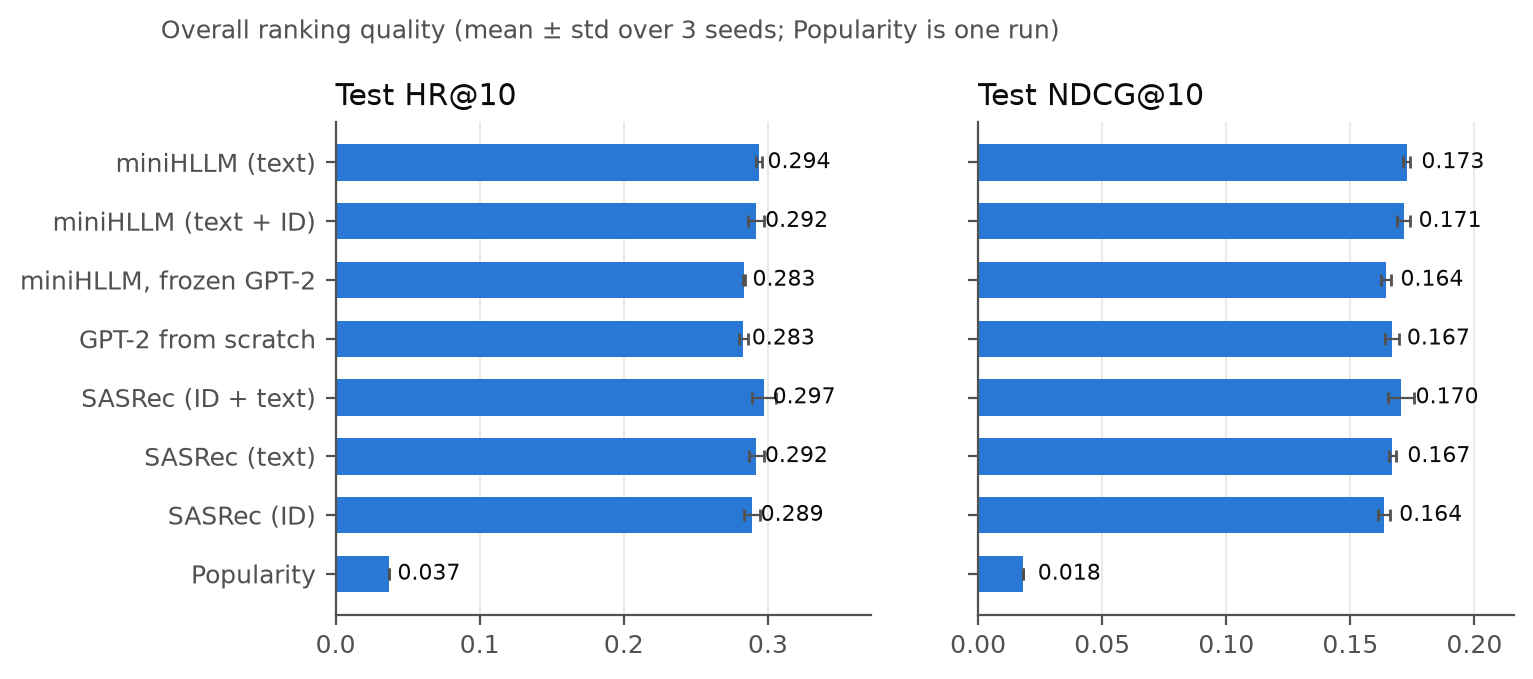
\includegraphics[width=\linewidth]{figures/overall_metrics.png}
\caption{测试集 HR@10 与 NDCG@10, 误差线为三种子样本标准差.}
\label{fig:overall}
\end{figure}

所有学习模型的 NDCG@10 都在热门推荐的 9 倍以上. H1 的 NDCG@10 与 NDCG@20 均值最高, 但与 S3, H4 的差距都在一个标准差内; HR@10 均值最高的是 S3. H1 三个种子的 NDCG@10 标准差为 0.001, 是各模型中最小的; SASRec 系列在 0.002 到 0.005 之间. H1 与 SASRec 的参数量相差约 200 倍, 见第~\ref{sec:limits} 节.

\subsection{收敛速度}

\begin{figure}[htbp]
\centering
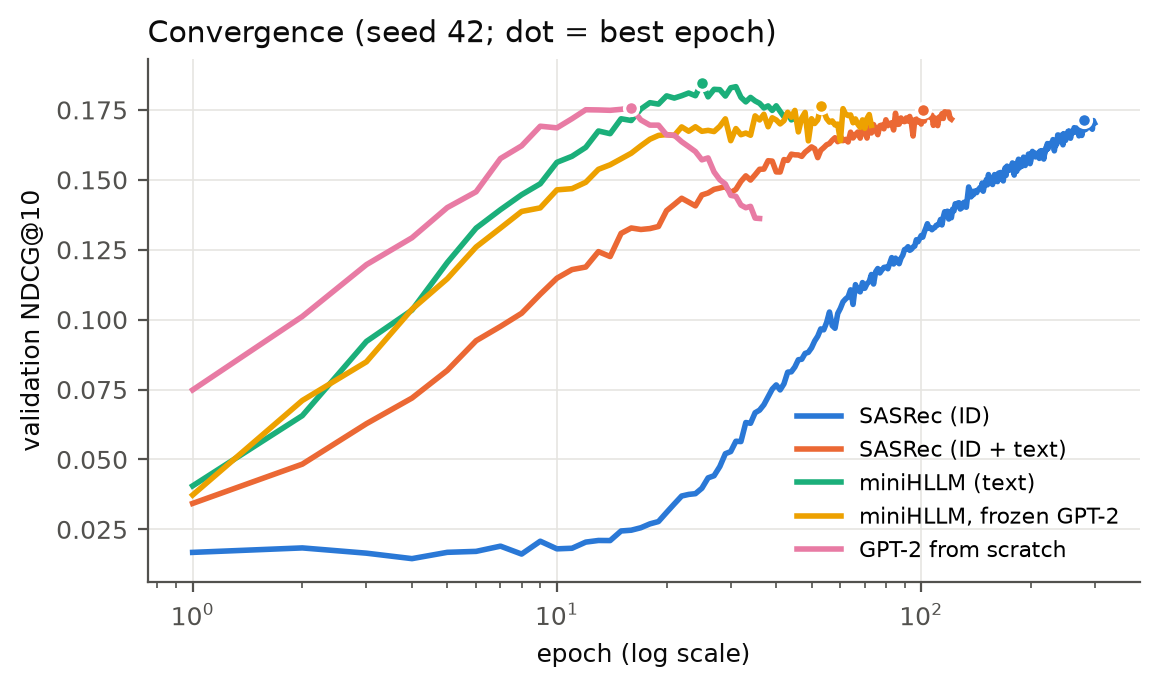
\includegraphics[width=\linewidth]{figures/training_curves.png}
\caption{种子 42 的验证集 NDCG@10 随训练轮次的变化, 横轴为对数刻度, 圆点为早停选中的最佳轮.}
\label{fig:curves}
\end{figure}

各模型的收敛速度差别很大 (图~\ref{fig:curves}). SASRec (ID) 的验证指标前 15 轮几乎不变, 之后缓慢上升, 最佳轮次在 250 到 300 之间. miniHLLM 第 1 轮就达到 SASRec (ID) 第 30 轮的水平, 25 轮达到最佳, 之后开始过拟合. 随机初始化的 GPT-2 上升最快, 约 15 轮达到峰值后迅速过拟合, 峰值低于预训练版本. 冻结 GPT-2 的版本上升平缓, 约 50 轮达到最佳, 之后保持稳定.

按墙钟时间, miniHLLM 一次训练约 15 分钟 (约 45 轮, 含早停等待的 20 轮), SASRec (ID) 约 3.5 分钟 (约 300 轮). miniHLLM 每轮耗时约为 SASRec (ID) 的 30 倍, 所需轮次约为其 1/6.

\subsection{冷门电影分析}

\begin{table}[htbp]
\centering
\caption{按目标电影训练热度分桶的测试 NDCG@10}
\label{tab:cold}
\footnotesize
\begin{tabular}{lrrr}
\toprule
模型 & $<100$ ($n$=507) & 100--500 ($n$=2,195) & $\geq 500$ ($n$=3,338) \\
\midrule
P\ \ Popularity & 0.000 & 0.000 & 0.033 \\
S1 SASRec (ID) & 0.052 $\pm$ 0.004 & 0.119 $\pm$ 0.005 & 0.210 $\pm$ 0.003 \\
S2 SASRec (text) & 0.042 $\pm$ 0.004 & 0.118 $\pm$ 0.004 & 0.218 $\pm$ 0.004 \\
S3 SASRec (ID + text) & 0.063 $\pm$ 0.005 & 0.123 $\pm$ 0.006 & 0.218 $\pm$ 0.006 \\
H2 GPT-2 scratch & 0.043 $\pm$ 0.004 & 0.113 $\pm$ 0.002 & 0.221 $\pm$ 0.005 \\
H3 miniHLLM (frozen) & \textbf{0.065 $\pm$ 0.006} & \textbf{0.124 $\pm$ 0.004} & 0.206 $\pm$ 0.005 \\
H4 miniHLLM (text + ID) & 0.046 $\pm$ 0.005 & 0.122 $\pm$ 0.003 & 0.223 $\pm$ 0.007 \\
H1 miniHLLM (text) & 0.043 $\pm$ 0.003 & 0.119 $\pm$ 0.004 & \textbf{0.228 $\pm$ 0.005} \\
\bottomrule
\end{tabular}
\end{table}

\begin{figure}[htbp]
\centering
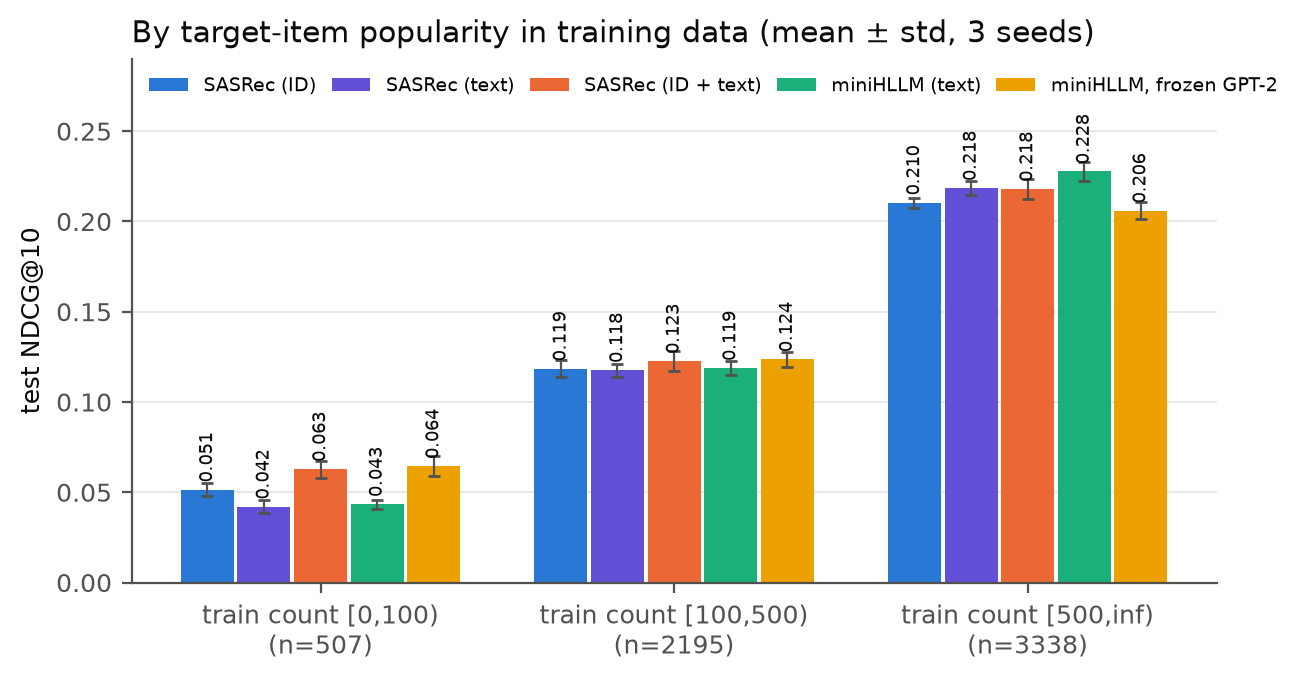
\includegraphics[width=\linewidth]{figures/coldstart_buckets.png}
\caption{各热度桶的测试 NDCG@10.}
\label{fig:cold}
\end{figure}

热门推荐在前两桶的 NDCG@10 为 0, 冷门目标只能靠个性化模型命中. 表~\ref{tab:cold} 有三点值得说明:
\begin{enumerate}
  \item \textbf{H1 的优势集中在热门桶.} H1 在 $\geq 500$ 桶的 NDCG@10 为 0.228, 比 SASRec (ID) 高 9\%; 在 $<100$ 桶为 0.043, 低于 SASRec (ID) 的 0.052. 一种可能的解释是全参数微调把模型容量用在了交互多的热门电影上.
  \item \textbf{H3 的情况相反.} 冻结 GPT-2, 只训练 1.8M 参数的 H3 在冷门桶为 0.065, 是各模型中最高的, 在热门桶则最低. H3 与 SASRec (ID) 的整体指标相同, 但 H3 在冷门桶更强, SASRec (ID) 在热门桶更强.
  \item \textbf{在 SASRec 骨干上, 文本要与 ID 一起用才对冷门桶有帮助.} 仅用文本的 S2 在冷门桶 (0.042) 低于仅用 ID 的 S1 (0.052), 二者相加的 S3 达到 0.063. 一种可能的解释是: 冷门桶的上限是 100 次交互, ID 向量在这一范围内仍能学到有用信息; 而在仅文本的模型中, 所有电影共用一个适配器, 冷门电影若与某部热门电影的标题或类型相近, 向量会被拉向后者. S2 与 H1 在冷门桶的结果几乎相同 (0.042 与 0.043), 说明这一弱势来自仅文本的电影表示, 而不是 GPT-2 骨干.
\end{enumerate}
冷门桶只有 507 位用户, 以上差异的统计功效有限.

\subsection{消融分析: 回答三个研究问题}

\textbf{Q1: 文本表示能否替代 ID?} 不含 ID 的 H1 测试 NDCG@10 为 $0.173 \pm 0.001$, 高于仅用 ID 的 S1 ($0.164 \pm 0.002$), 与使用 ID 和文本的 S3 ($0.170 \pm 0.005$) 相差不到一个标准差. 在 H1 上加回 ID (H4, $0.172 \pm 0.003$) 没有可见变化, 冷门桶从 0.043 变为 0.046. 因此在 ML-1M 上, 只用标题和类型的文本表示即可达到含 ID 模型的水平; 能否超过, 三个种子不足以判断.

\textbf{Q2: 语言预训练能否迁移?} H1 与 H2 结构相同, 只差初始化. 预训练版本的 NDCG@10 为 $0.173 \pm 0.001$, 随机初始化在两个学习率下分别为 $0.167 \pm 0.003$ 和 $0.166 \pm 0.001$, 差距是种子标准差的 2 到 7 倍. 随机初始化的模型约 15 轮即开始过拟合, 预训练模型到 25 轮才达到最佳. GPT-2 只在网页文本上预训练过, 这一结果说明从文本中学到的权重对行为序列建模也有帮助.

\textbf{Q3: 微调程度与冷门电影的关系?} 冻结的 H3 (1.8M 可训练参数) 冷门桶最好, 热门桶最差; 全参数微调的 H1 (87.6M) 热门桶最好, 冷门桶较差; 二者整体 NDCG@10 相差 0.009. 微调程度决定了模型偏向热门还是冷门电影. 本项目没有测试 LoRA 等介于两者之间的方案.

\subsection{推荐案例}

用户 1 测试序列的最后五部为 \emph{A Bug's Life}, \emph{Antz}, \emph{The Hunchback of Notre Dame}, \emph{Hercules} 和 \emph{Mulan}, 真实的下一部是 \emph{Pocahontas}. 两个模型的 Top-10 推荐 (* 为命中):

\begin{center}
\footnotesize
\begin{tabular}{rll}
\toprule
排名 & miniHLLM (text) & SASRec (ID) \\
\midrule
1 & Lion King, The (1994) & Prince of Egypt, The (1998) \\
2 & Prince of Egypt, The (1998) & Lion King, The (1994) \\
3 & Anastasia (1997) & Anastasia (1997) \\
4 & \textbf{* Pocahontas (1995)} & \textbf{* Pocahontas (1995)} \\
5 & Little Mermaid, The (1989) & South Park: Bigger, Longer and Uncut (1999) \\
6 & Jungle Book, The (1967) & Alice in Wonderland (1951) \\
7 & Alice in Wonderland (1951) & Beavis and Butt-head Do America (1996) \\
8 & Robin Hood (1973) & Stuart Little (1999) \\
9 & Balto (1995) & Sword in the Stone, The (1963) \\
10 & Lady and the Tramp (1955) & Fantasia 2000 (1999) \\
\bottomrule
\end{tabular}
\end{center}

两个模型都在第 4 位命中. miniHLLM 的 10 部都是家庭向动画片, 与用户近期观看的一致; SASRec (ID) 的列表中则有 \emph{South Park} 和 \emph{Beavis and Butt-head} 两部成人动画. 这两部片的类型标注中没有 Children's, 而 miniHLLM 的电影向量由标题和类型文本计算, 能把它们与儿童动画区分开.

\section{项目总结}

\subsection{主要成果}

\begin{enumerate}
  \item 第一部分实现了课程框架的 GPT-2 + NCF. 第二部分实现了 miniHLLM, 把 HLLM 的分层 LLM 结构改造为 GPT-2 small 版本, 可在单卡上训练, 代码约 550 行, 训练一次约 15 分钟.
  \item 在统一的时间 leave-one-out 划分与全量排序评测下, 比较了 8 个模型, 每个 3 个种子, 共 28 次训练, 并按目标电影热度分桶评测. 全部日志, 逐轮曲线与指标存放在 \texttt{recommender/miniHLLM/results/main/}.
  \item 不含 ID 的 miniHLLM 达到了含 ID 的 SASRec 的水平, 种子间方差最小, 收敛最快; 同结构下预训练初始化比随机初始化的 NDCG@10 高 0.006; 在 miniHLLM 上加 ID 没有可见变化; 微调程度决定模型偏向热门还是冷门电影.
  \item 处理了两个影响结果正确性的实现问题: GPT-2 特征的各向异性, 以及 bf16 评测中同分导致的指标虚高.
\end{enumerate}

\subsection{不足}
\label{sec:limits}

\begin{itemize}
  \item \textbf{电影文本信息量小.} 只有标题和类型, 平均十几个 token, 限制了文本分支的上限, 可能也是仅文本模型在冷门桶较弱的原因之一.
  \item \textbf{Item LLM 没有微调.} HLLM 端到端训练两个 LLM; 本项目受显存限制, 只在冻结特征上训练适配器, 没有验证电影侧与用户侧的联合优化.
  \item \textbf{参数量不对等.} miniHLLM 有 87M 参数, SASRec 只有 0.4M, 相差约 200 倍. H2 对照只隔离了初始化, H1 与 S3 的差别不能单独归因于预训练或结构. 加入一个参数量接近 GPT-2, 从零训练的 SASRec 会使比较更公平.
  \item \textbf{没有评测真正的冷启动.} 本项目的冷门桶指训练中出现少于 100 次的电影, 没有评测训练中零交互的新电影.
  \item \textbf{数据集单一且偏小.} ML-1M 的冷门桶只有 507 位用户, 统计功效有限; 结论能否推广到更大, 更稀疏的数据集未知.
  \item \textbf{微调程度只测了冻结与全参数两种.} 没有测试 LoRA, 只微调顶层等中间方案.
\end{itemize}

\subsection{改进方向}
\label{sec:future}

\begin{enumerate}
  \item \textbf{用生成式 LLM 丰富电影文本.} 用本地指令模型为每部电影生成剧情简介, 风格与受众描述后再编码, 可能提升文本分支在冷门桶上的表现.
  \item \textbf{Item LLM 的参数高效微调.} 对电影侧 GPT-2 加 LoRA, 每步只对 batch 内出现的电影重新编码, 其余使用缓存向量, 使两个 LLM 的联合训练在单卡上可行.
  \item \textbf{连续改变微调程度.} 在冻结与全参数之间加入 LoRA 秩 8, 16, 64 和只微调顶部 $k$ 层, 画出整体指标与冷门桶指标随可训练参数量的变化, 定量回答 Q3.
  \item \textbf{等参数量对照与更大数据集.} 增加与 GPT-2 同规模, 从零训练的 Transformer, 并在 Amazon Reviews 等物品更多, 更稀疏的数据集上验证.
  \item \textbf{与生成式推荐对比.} 在相同的电影文本向量上训练 RQ-VAE 得到语义 ID, 实现 TIGER 风格的生成式检索, 与 miniHLLM 的稠密检索对比.
\end{enumerate}

\section*{附录: 复现}

\begin{footnotesize}
\begin{verbatim}
git lfs pull                       # 数据, GPT-2 权重
cd recommender/miniHLLM
python item_features.py            # 电影文本向量 -> weight/item_text_features.pt
./run_all.sh && ./run_extra.sh     # 28 次训练 -> results/main/
python summarize.py                # 汇总表
python plot_results.py             # 图 -> figures/
\end{verbatim}
\end{footnotesize}

第一部分:
\begin{footnotesize}
\begin{verbatim}
cd recommender/base_LLM_NCF
python gpt2.py && python main.py --epochs 3
\end{verbatim}
\end{footnotesize}

\section*{参考文献}

\begin{itemize}
  \item Chen, J. et al. HLLM: Enhancing Sequential Recommendations via Hierarchical Large Language Models for Item and User Modeling. arXiv:2409.12740, 2024.
  \item Kang, W.-C. \& McAuley, J. Self-Attentive Sequential Recommendation. ICDM 2018.
  \item He, X. et al. Neural Collaborative Filtering. WWW 2017.
  \item Rendle, S. et al. BPR: Bayesian Personalized Ranking from Implicit Feedback. UAI 2009.
  \item Radford, A. et al. Language Models are Unsupervised Multitask Learners. OpenAI, 2019.
  \item Ethayarajh, K. How Contextual are Contextualized Word Representations? EMNLP 2019.
  \item Timkey, W. \& van Schijndel, M. All Bark and No Bite: Rogue Dimensions in Transformer Language Models Obscure Representational Quality. EMNLP 2021.
  \item Rajput, S. et al. Recommender Systems with Generative Retrieval. NeurIPS 2023.
\end{itemize}

\end{document}
